%----------------------------------------------------------------------
% 實驗設計分析
%----------------------------------------------------------------------

\chapter{Evaluation}\label{sec:evalutaion}
\section{Experiment }\label{sec:3-experiment}
\subsection{Experiment Setup}\label{sec:3-setup}
Our experiments aim to illustrate how the strengths of one sensor compensate for weaknesses in the other, 
demonstrating the potential of sensor fusion.
The weakness inherent in radar lies in its challenge to recognize objects due to sparse measurements. 
Although a camera offers high-resolution measurements, 
it lacks depth perception. 
However, radar compensates for this limitation by providing highly accurate range measurements, 
effectively mitigating the shortcomings of the camera.
To test the performance of the algorithm, 3 specific scenarios were tested:
1. Control scenario, when object 1 (white) and object 2 (yellow) do not crosspath.
2. One object conceals another and continues their original trajectory after departing.
3. One object conceals another and changes trajectory when departing.
\begin{figure}[!htb]
    \centering
    \begin{subfigure}{0.25\linewidth}
        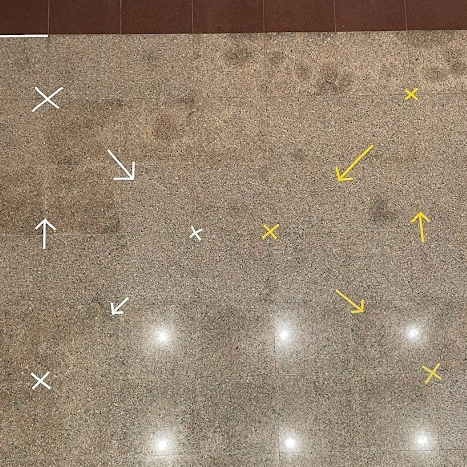
\includegraphics[width=5.5cm]{Figures/scenario_1_gt.png}
        \caption{scenario 1}
        \label{subfig:scenario1gt}
    \end{subfigure}
    \hfill
    \begin{subfigure}{0.25\linewidth}
        \centering
        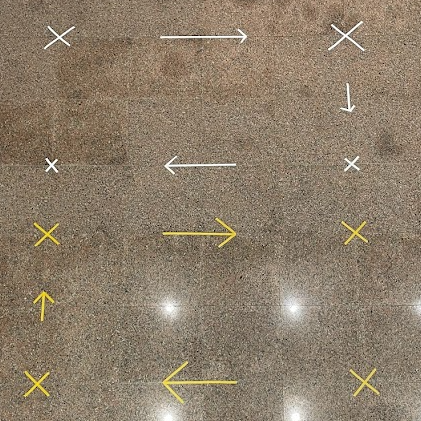
\includegraphics[width=5.5cm]{Figures/scenario_2_gt.png}
        \caption{scenario 2}
        \label{subfig:scenario2gt}
    \end{subfigure}
    \hfill
    \begin{subfigure}{0.25\linewidth}
        \centering
        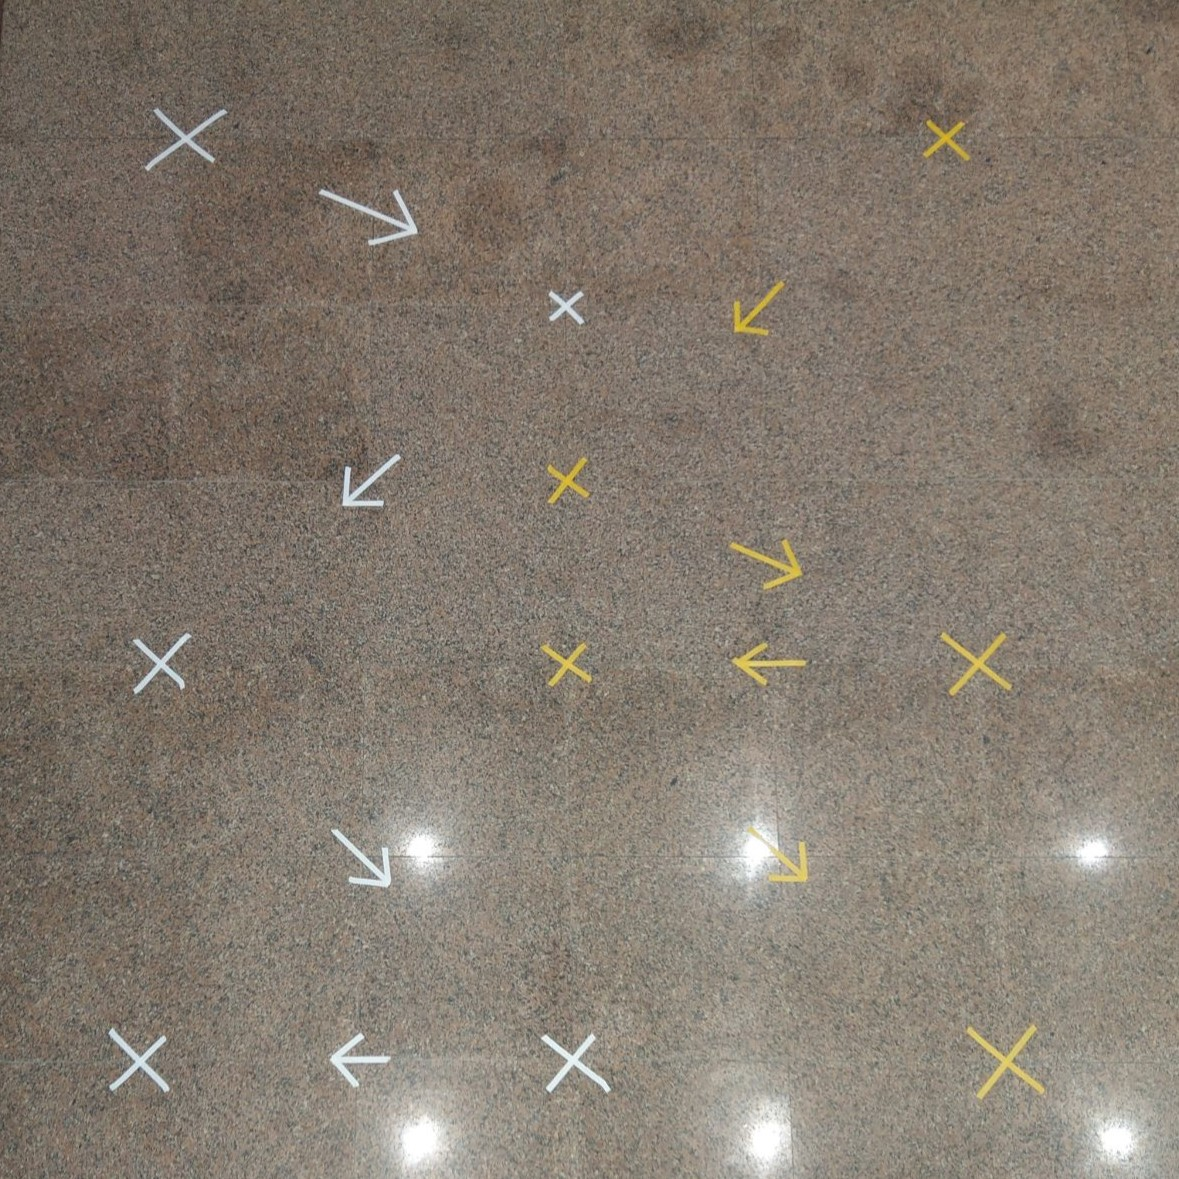
\includegraphics[width=5.5cm]{Figures/scenario_3_gt.jpg}
        \caption{scenario 3}
        \label{subfig:scenario3gt}
    \end{subfigure}

    \caption{Bird Eye View of multi-object tracking experiments' ground truth}
    \label{fig:ground_truth}
\end{figure}

\subsection{Challenges to Overcome}\label{sec:3-challenge}
Blind spot of both sensors.
Challenges the algorithm to correctly predict objects when data is obstructed.

\begin{figure}[!htb]
    \centering
    \begin{subfigure}{0.3\linewidth}
        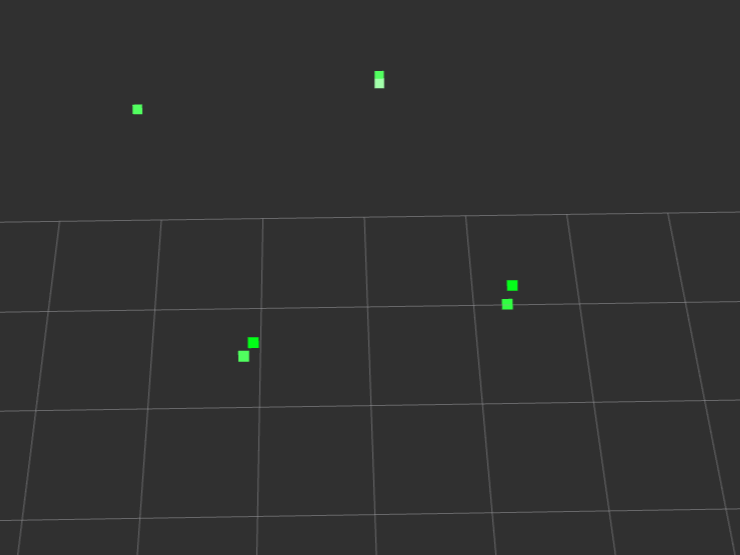
\includegraphics[width=7cm]{Figures/before_conceal_radar.png}
        \caption{Raw radar data}
        \label{subfig:before_conceal_radar_fig}
    \end{subfigure}
    \hspace{0.15\textwidth}
    %\hfill
    \begin{subfigure}{0.3\linewidth}
        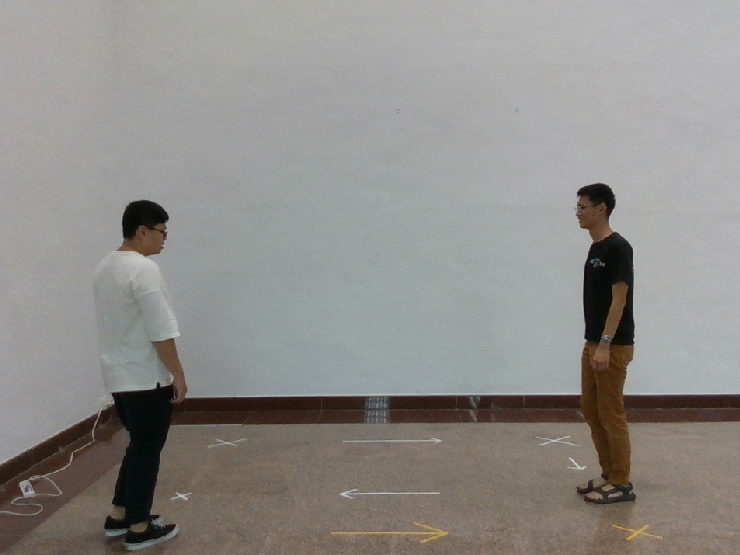
\includegraphics[width=7cm]{Figures/before_conceal_image.png}
        \caption{Image frame}
        \label{subfig:before_conceal_image_fig}
    \end{subfigure}

    \caption{Object 1 and object 2 before crossingpath}
    \label{fig:before_conceal_fig}
\end{figure}

From figure \ref*{fig:concealing_fig}\subref{subfig:concealing_radar_fig} can be seen that both object clusters disappear.



\begin{figure}[!htb]
    \centering
    \begin{subfigure}{0.3\linewidth}
        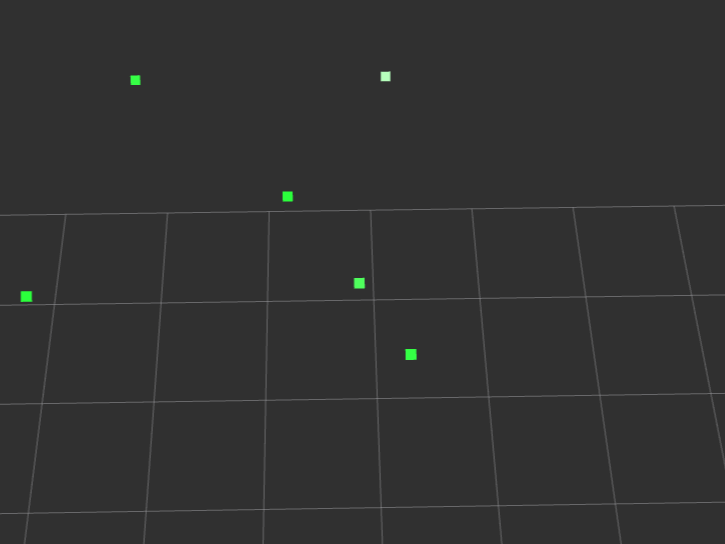
\includegraphics[width=7cm]{Figures/concealing_radar.png}
        \caption{Raw radar data}
        \label{subfig:concealing_radar_fig}
    \end{subfigure}
    \hspace{0.15\textwidth}
    %\hfill
    \begin{subfigure}{0.3\linewidth}
        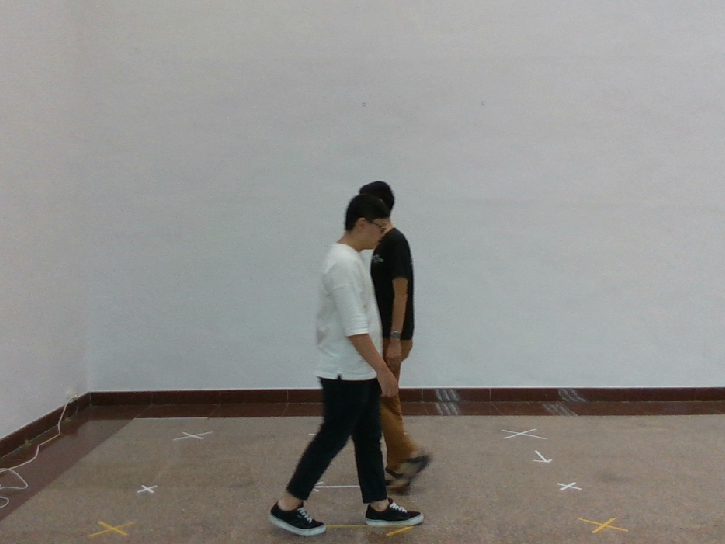
\includegraphics[width=7cm]{Figures/concealing_image.png}
        \caption{Image frame}
        \label{subfig:concealing_image_fig}
    \end{subfigure}

    \caption{Object 1 covers object 2}
    \label{fig:concealing_fig}
\end{figure}

\begin{figure}[!htb]
    \centering
    \begin{subfigure}{0.3\linewidth}
        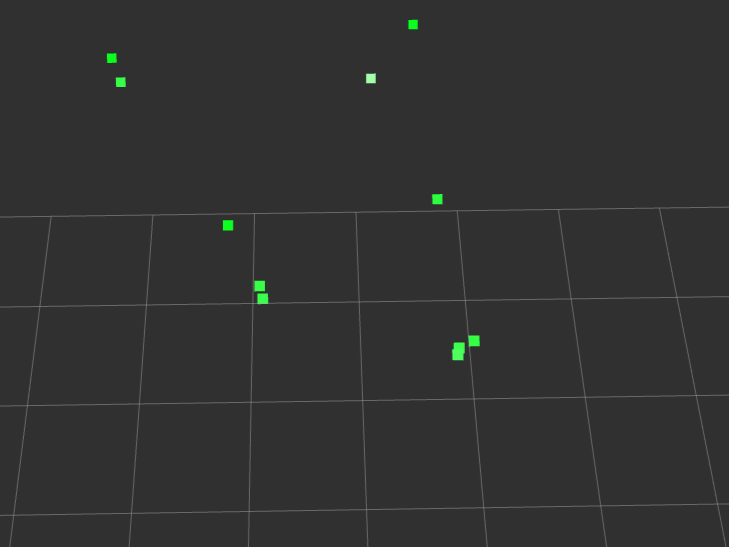
\includegraphics[width=7cm]{Figures/after_conceal_radar.png}
        \caption{Raw radar data}
        \label{subfig:after_conceal_radar_fig}
    \end{subfigure}
    \hspace{0.15\textwidth}
    %\hfill
    \begin{subfigure}{0.3\linewidth}
        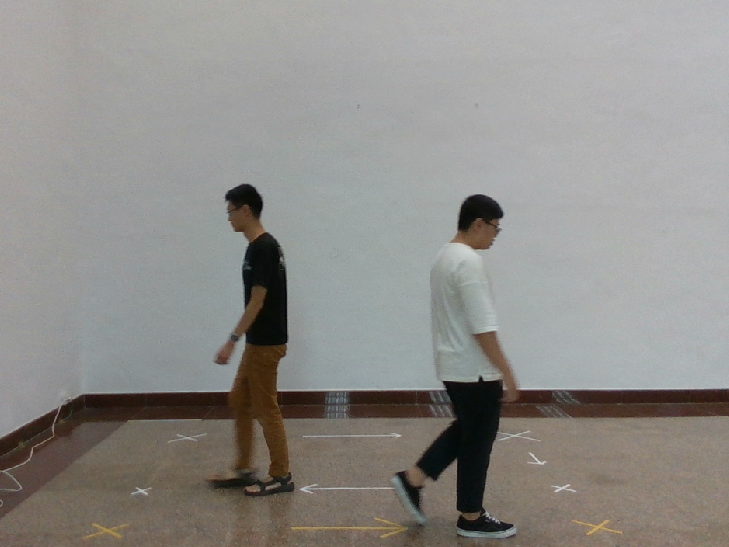
\includegraphics[width=7cm]{Figures/after_conceal_image.png}
        \caption{Image frame}
        \label{subfig:after_conceal_image_fig}
    \end{subfigure}

    \caption{Object 1 and object 2 seperates}
    \label{fig:after_conceal_fig}
\end{figure}





\vspace*{5cm}
\section{Experiment Result}\label{sec:3-exp_result}
\subsection{Scenario 1}\label{sec:3-exp_result1}
Scenario 1 is the control when object 1 and object 2 do not crosspath.
\href{https://drive.google.com/file/d/1SL30CC6EpyI4NLOcGnfALKAP44P82u9n/view?usp=sharing}{\color{blue}{Video}}
\begin{figure}[!htb]
    \centering
    \begin{subfigure}[b]{0.475\textwidth}%{0.25\linewidth}
        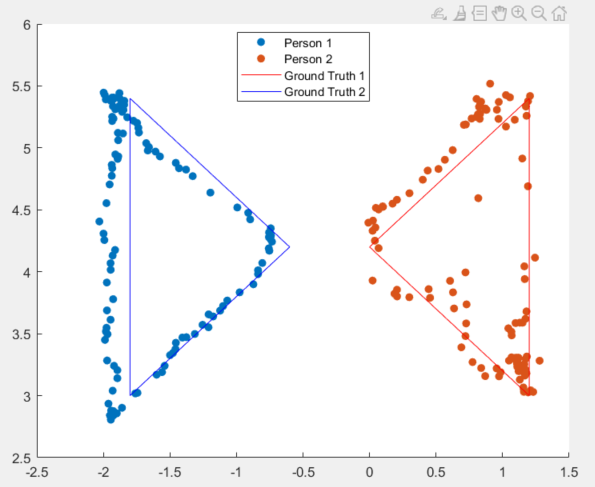
\includegraphics[width=7cm]{Figures/1_before.png}
        \caption{Only radar object tracking}
        \label{subfig:without_fusion_1}
    \end{subfigure}
    %\hspace{0.15\textwidth}
    \hfill
    \begin{subfigure}[b]{0.475\textwidth}%{0.25\linewidth}
        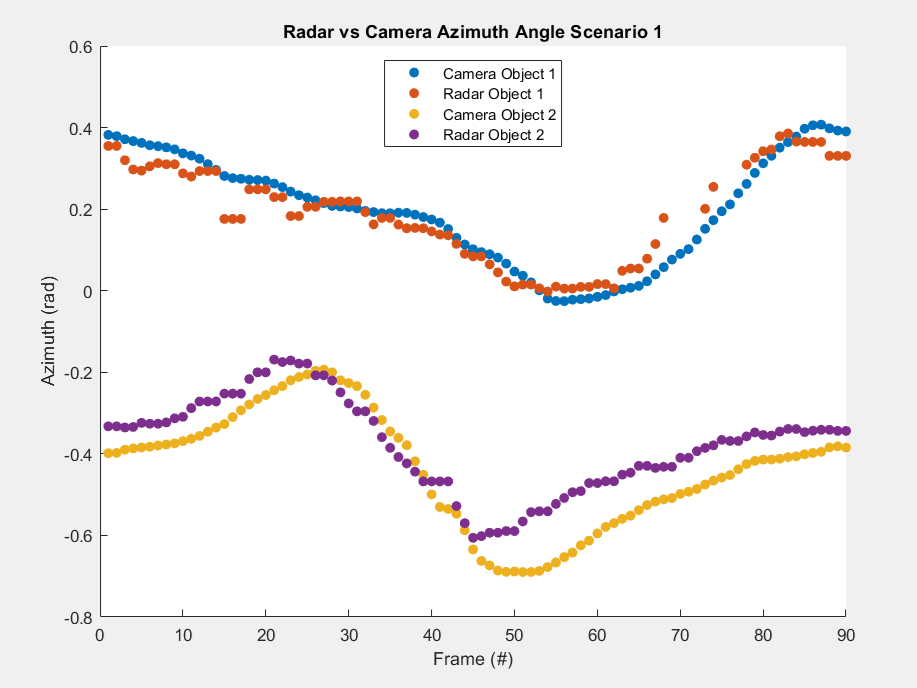
\includegraphics[width=7cm]{Figures/rad_v_cam_1.png}
        \caption{Raw radar and image data after data association}
        \label{subfig:raw_fusion_1}
    \end{subfigure}
    %\hfill
    \vskip\baselineskip

    \begin{subfigure}[b]{0.475\textwidth}%{0.25\linewidth}
        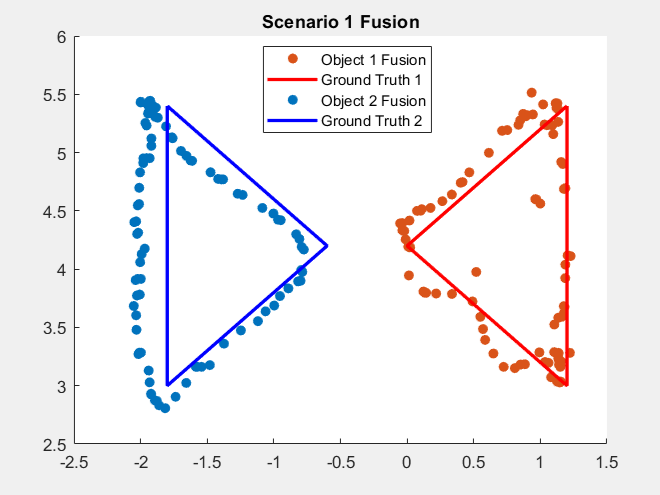
\includegraphics[width=7cm]{Figures/fusion_scene1.png}
        \caption{Fused data}
        \label{subfig:fusion_1}
    \end{subfigure}

    \begin{subfigure}[b]{0.475\textwidth}%{0.25\linewidth}
        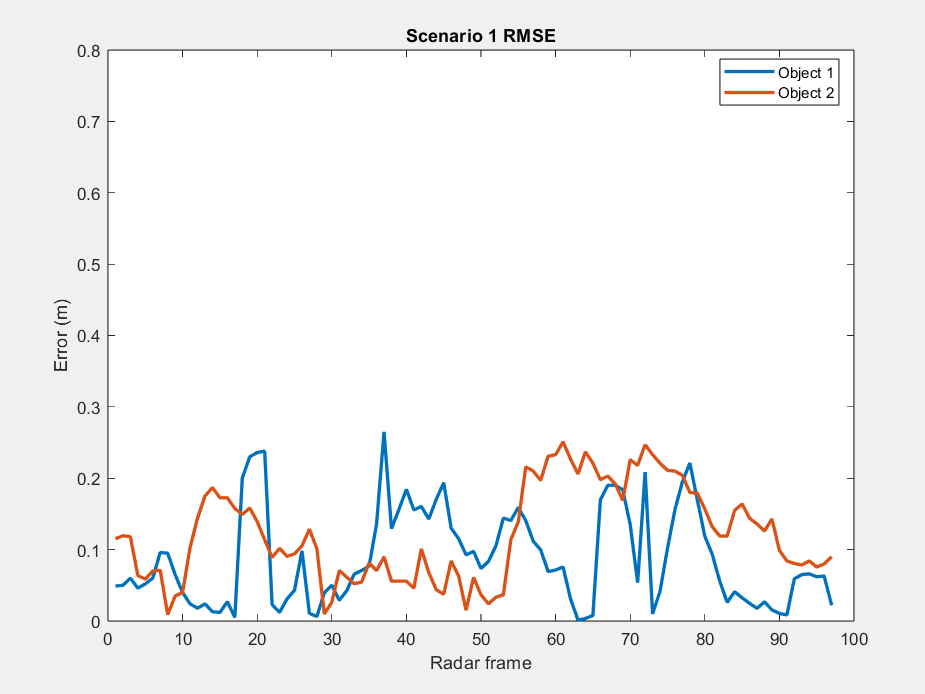
\includegraphics[width=7cm]{Figures/RMSE1.png}
        \caption{RMSE to ground truth}
        \label{subfig:RMSE_1}
    \end{subfigure}

    \caption{Scenario 1 multi-object tracking}
    \label{fig:scenario_result_1}
\end{figure}

\subsection{Scenario 2}\label{sec:3-exp_result2}
In scenario 2, object 1 crosses path with object 2 in a straight line horizontally.
After concealing object 2 from both camera and radar, both objects continue their original trajectory.
In figure \ref*{fig:scenario_result_2}\subref{subfig:without_fusion_2} can be seen that object 1 and object 2 switch places.
The algorithm is able to track and identify objects 1 and 2 correctly (figure \ref*{fig:scenario_result_2}\subref{subfig:with_fusion_2}).
\href{https://drive.google.com/file/d/1YnliV7YRzahYNpIehctzrNrf0Z0ZpIeY/view?usp=sharing}{\color{blue}{Video}}
\begin{figure}[!htb]
    \centering
    \begin{subfigure}[b]{0.475\textwidth}%{0.25\linewidth}
        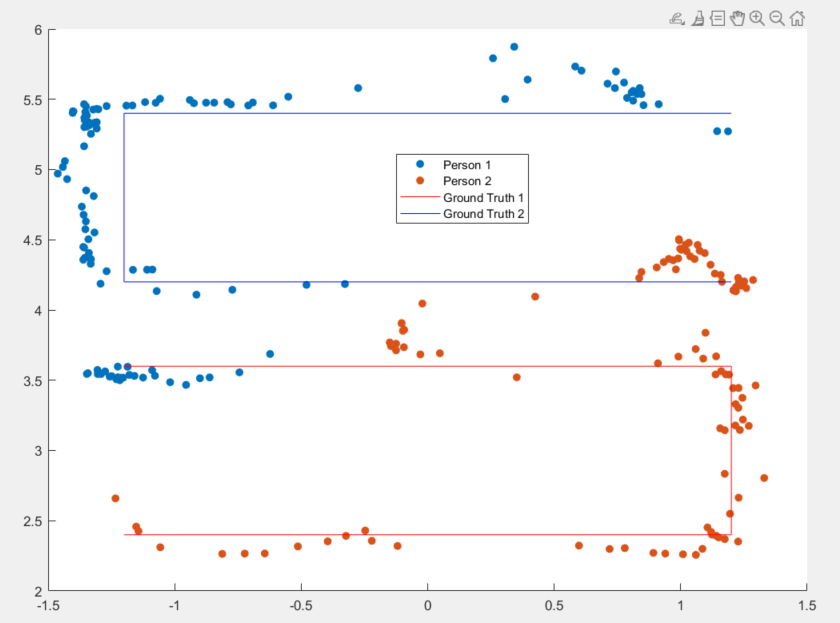
\includegraphics[width=7cm]{Figures/2_before.png}
        \caption{Only radar object tracking}
        \label{subfig:without_fusion_2}
    \end{subfigure}
    %\hspace{0.15\textwidth}
    \hfill
    \begin{subfigure}[b]{0.475\textwidth}%{0.25\linewidth}
        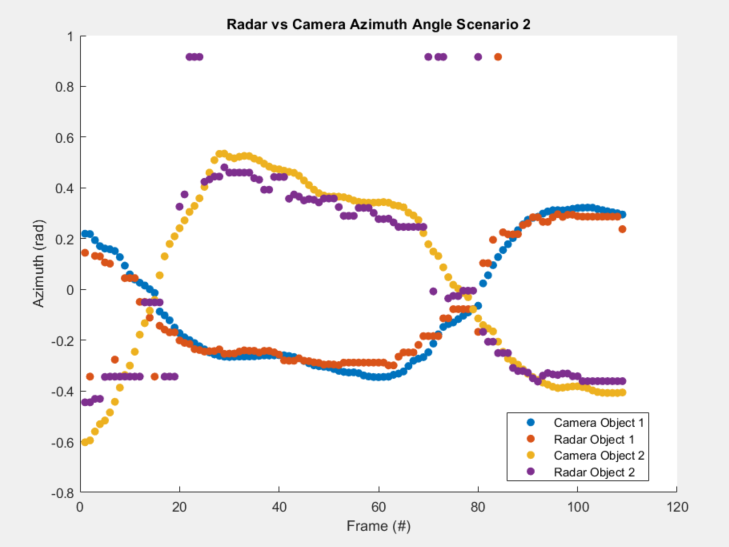
\includegraphics[width=7cm]{Figures/rad_v_cam_2.png}
        \caption{Raw radar and image data after data association}
        \label{subfig:raw_fusion_2}
    \end{subfigure}
    %\hfill
    \vskip\baselineskip

    \begin{subfigure}[b]{0.475\textwidth}%{0.25\linewidth}
        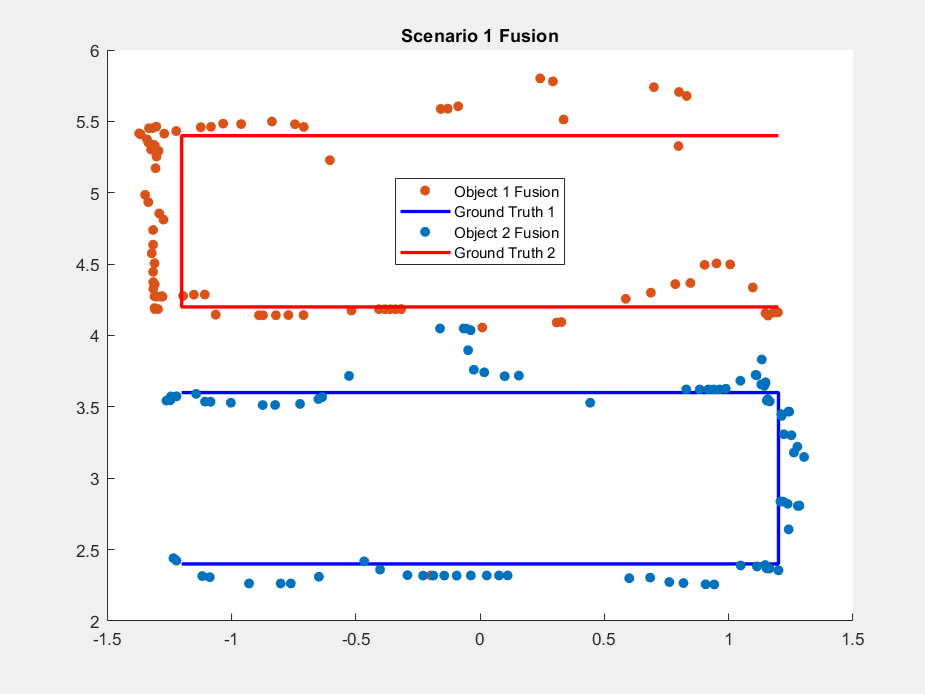
\includegraphics[width=7cm]{Figures/fusion_scene2.png}
        \caption{Fused data}
        \label{subfig:with_fusion_2}
    \end{subfigure}
    \begin{subfigure}[b]{0.475\textwidth}%{0.25\linewidth}
        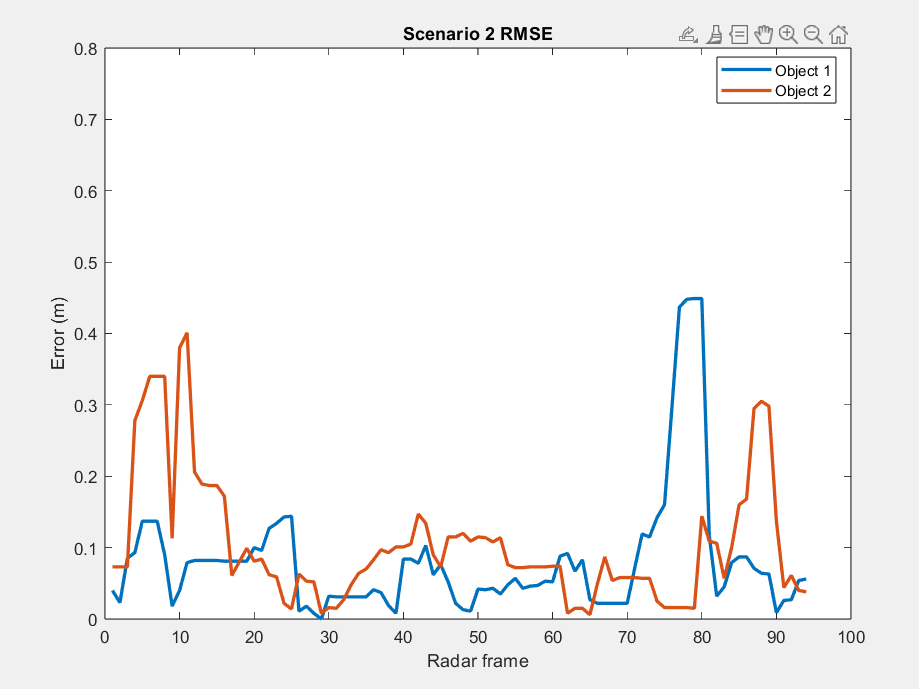
\includegraphics[width=7cm]{Figures/RMSE2.png}
        \caption{RMSE to ground truth}
        \label{subfig:RMSE_2}
    \end{subfigure}
    \caption{Scenario 2 multi-object tracking}
    \label{fig:scenario_result_2}
\end{figure}
\newpage
\subsection{Scenario 3}\label{sec:3-exp_result3}
In scenario 3, object 1 covers object 2, and in the next few frames, object 2 covers object 1.
In this scenario, both objects change trajectory when departing from each other.
In figure \ref*{fig:scenario_result_3}\subref{subfig:without_fusion_3} can be seen that object 1 and object 2 switch places.
The algorithm is able to track and identify objects 1 and 2 correctly (figure \ref*{fig:scenario_result_3}\subref{subfig:with_fusion_3}).
\href{https://drive.google.com/file/d/1bd92Bu6CJeL1QIIbBlW42cAozxEcis-d/view?usp=sharing}{\color{blue}{Video}}
\begin{figure}[!htb]
    \centering
    %\begin{adjustwidth}{-8em}{0em}
    \begin{subfigure}[b]{0.475\textwidth}%{0.25\linewidth}
        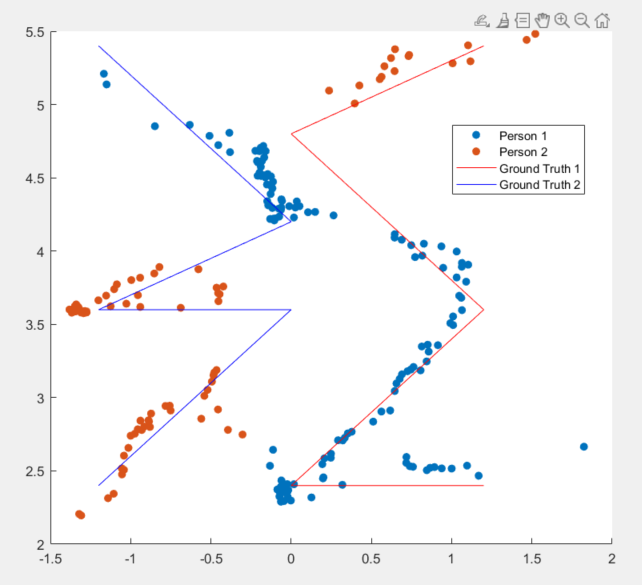
\includegraphics[width=7cm]{Figures/3_before.png}
        \caption{Only radar object tracking}
        \label{subfig:without_fusion_3}
    \end{subfigure}
    %\hspace{0.05\textwidth}
    \hfill
    \begin{subfigure}[b]{0.475\textwidth}%{0.25\linewidth}
        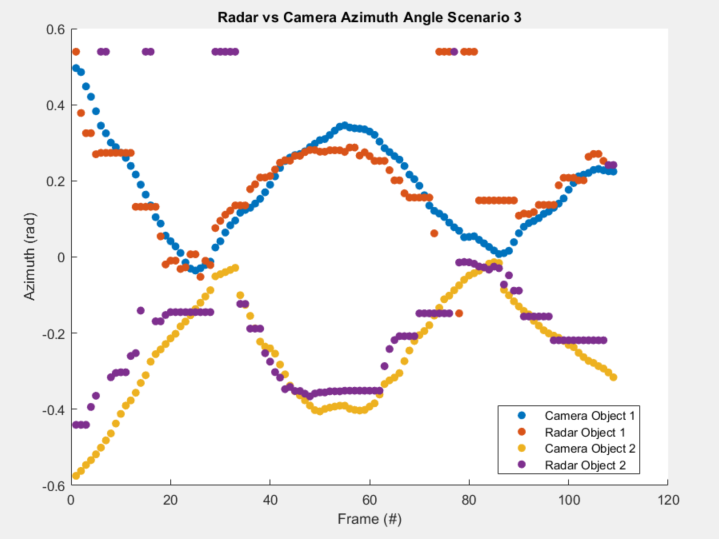
\includegraphics[width=7cm]{Figures/rad_v_cam_3.png}
        \caption{Raw radar and image data after data association}
        \label{subfig:raw_fusion_3}
    \end{subfigure}
    \vskip\baselineskip
%\end{adjustwidth}
    %\hfill
    %\hspace{0.05\textwidth}

    \begin{subfigure}[b]{0.475\textwidth}%{0.25\linewidth}
        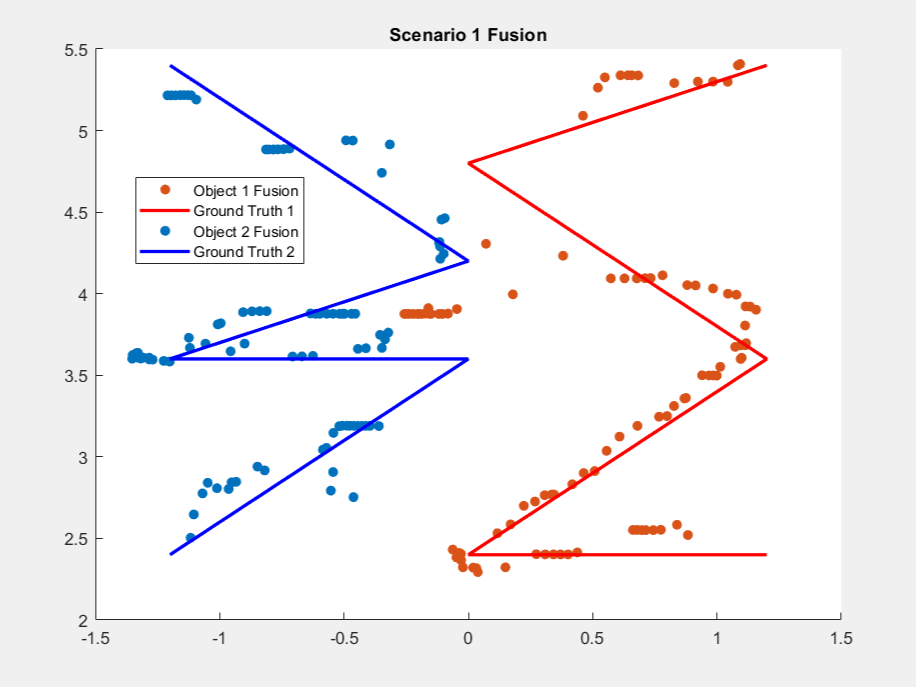
\includegraphics[width=7cm]{Figures/fusion_scene3.png}
        \caption{Fused data}
        \label{subfig:with_fusion_3}
    \end{subfigure}
    \begin{subfigure}[b]{0.475\textwidth}%{0.25\linewidth}
        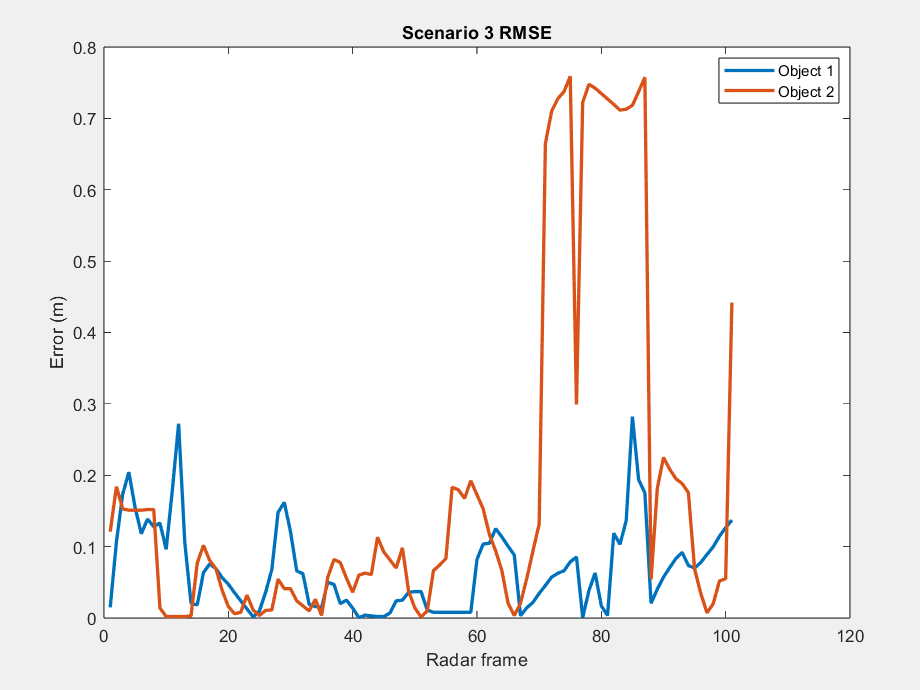
\includegraphics[width=7cm]{Figures/RMSE3.png}
        \caption{RMSE to ground truth}
        \label{subfig:RMSE_3}
    \end{subfigure}
    \caption{Scenario 3 multi-object tracking}
    \label{fig:scenario_result_3}
\end{figure}
\newpage



\section{Error Evaluation}\label{sec:3-evaluation}
\begin{equation}\label{equ:4_RMSE}
\text{RMSE} = \sqrt{\frac{1}{n}\sum_{i=1}^{n}(y_i - \hat{y}_i)^2}
\end{equation}
From Scenario 1, it becomes apparent that all components—fusion, radar, 
or camera—deliver commendable performance. 
Although the camera slightly outperforms in x-axis accuracy. 
In scenario 2, where the algorithm showcases its strengths, 
it combines the best of both sensors to produce better a result.
Conversely, in Scenario 3, radar struggles significantly in tracking object 2 as it enters its blind spot. 
Nevertheless, the algorithm maintains its performance by incorporating camera data. 
The collective analysis across all scenarios yields an average RMSE of 0.1561m.
\begin{table}[h!]
    \begin{center}
      \label{tab:table2}
      \begin{tabular}{c|c|c|c|c|c|c} % <-- Alignments: 1st column left, 2nd middle and 3rd right, with vertical lines in between
        \multirow{3}{*}{\textbf{Scenario}} & \multicolumn{6}{c}{\textbf{RMSE (m)}}\\\cline{2-7}
                                            & \multicolumn{3}{c|}{\textbf{Object 1}}  & \multicolumn{3}{c}{\textbf{Object 2}}\\
        \cline{2-7}
                   & Fusion & Camera \tablefootnote{\label{note1}only lateral error}& Radar & Fusion & Camera\footref{note1} & Radar \\
        \hline
        Scenario 1 & 0.1388 & 0.1922 & \textbf{0.1124} & \textbf{0.105}  & 0.1236 & 0.1201 \\
        Scenario 2 & \textbf{0.1206} & 0.1211 & 0.1228 & \textbf{0.1687} & 0.1982 & 0.2014 \\
        Scenario 3 & \textbf{0.0903} & 0.1211 & 0.0928 & 0.3075 & \textbf{0.2381} & 0.3592 \\
      \end{tabular}
    \end{center}
    \caption{All scenarios RMSE compared}
    \label{tab:scenarios_rmse}
  \end{table}

  

Comparison of errors between the author's proposed method and other radar-camera tracking algorithms.
  \begin{table}[h!]
    \begin{center}
      \label{tab:table1}
      \begin{tabular}{l|c|c|c|l} % <-- Alignments: 1st column left, 2nd middle and 3rd right, with vertical lines in between
        \textbf{Method} & \textbf{Radar} & \textbf{Object} & \textbf{Max Range} & \textbf{RMSE} \\% %object detected
        \hline
        Proposed                           & AWR1843 & human   & 6m  & \textbf{0.1561 m}  \\%& 6m 
        \citeauthor{9081940}\cite{9081940} &  RT3002 & vehicle & 40m & 0.18 m \\%
        \citeauthor{method1}\cite{method1} & AWR1642 & vehicle & 50m & 0.1828 m\\%& 50m
        \citeauthor{8932892}\cite{8932892} & IWR1443 & human   & 6m  & 0.2486 m\\%
        \citeauthor{8844649}\cite{8844649} & AWR1642 & human   & 10m & 0.2902 m \\%
        
      \end{tabular}
    \end{center}
    \caption{Comparison of other tracking method}
    \label{tab:method_rmse}
  \end{table}


